\documentclass[twoside]{book}

% Packages required by doxygen
\usepackage{fixltx2e}
\usepackage{calc}
\usepackage{doxygen}
\usepackage[export]{adjustbox} % also loads graphicx
\usepackage{graphicx}
\usepackage[utf8]{inputenc}
\usepackage{makeidx}
\usepackage{multicol}
\usepackage{multirow}
\PassOptionsToPackage{warn}{textcomp}
\usepackage{textcomp}
\usepackage[nointegrals]{wasysym}
\usepackage[table]{xcolor}

% Font selection
\usepackage[T1]{fontenc}
\usepackage[scaled=.90]{helvet}
\usepackage{courier}
\usepackage{amssymb}
\usepackage{sectsty}
\renewcommand{\familydefault}{\sfdefault}
\allsectionsfont{%
  \fontseries{bc}\selectfont%
  \color{darkgray}%
}
\renewcommand{\DoxyLabelFont}{%
  \fontseries{bc}\selectfont%
  \color{darkgray}%
}
\newcommand{\+}{\discretionary{\mbox{\scriptsize$\hookleftarrow$}}{}{}}

% Page & text layout
\usepackage{geometry}
\geometry{%
  a4paper,%
  top=2.5cm,%
  bottom=2.5cm,%
  left=2.5cm,%
  right=2.5cm%
}
\tolerance=750
\hfuzz=15pt
\hbadness=750
\setlength{\emergencystretch}{15pt}
\setlength{\parindent}{0cm}
\setlength{\parskip}{3ex plus 2ex minus 2ex}
\makeatletter
\renewcommand{\paragraph}{%
  \@startsection{paragraph}{4}{0ex}{-1.0ex}{1.0ex}{%
    \normalfont\normalsize\bfseries\SS@parafont%
  }%
}
\renewcommand{\subparagraph}{%
  \@startsection{subparagraph}{5}{0ex}{-1.0ex}{1.0ex}{%
    \normalfont\normalsize\bfseries\SS@subparafont%
  }%
}
\makeatother

% Headers & footers
\usepackage{fancyhdr}
\pagestyle{fancyplain}
\fancyhead[LE]{\fancyplain{}{\bfseries\thepage}}
\fancyhead[CE]{\fancyplain{}{}}
\fancyhead[RE]{\fancyplain{}{\bfseries\leftmark}}
\fancyhead[LO]{\fancyplain{}{\bfseries\rightmark}}
\fancyhead[CO]{\fancyplain{}{}}
\fancyhead[RO]{\fancyplain{}{\bfseries\thepage}}
\fancyfoot[LE]{\fancyplain{}{}}
\fancyfoot[CE]{\fancyplain{}{}}
\fancyfoot[RE]{\fancyplain{}{\bfseries\scriptsize Generated by Doxygen }}
\fancyfoot[LO]{\fancyplain{}{\bfseries\scriptsize Generated by Doxygen }}
\fancyfoot[CO]{\fancyplain{}{}}
\fancyfoot[RO]{\fancyplain{}{}}
\renewcommand{\footrulewidth}{0.4pt}
\renewcommand{\chaptermark}[1]{%
  \markboth{#1}{}%
}
\renewcommand{\sectionmark}[1]{%
  \markright{\thesection\ #1}%
}

% Indices & bibliography
\usepackage{natbib}
\usepackage[titles]{tocloft}
\setcounter{tocdepth}{3}
\setcounter{secnumdepth}{5}
\makeindex

% Hyperlinks (required, but should be loaded last)
\usepackage{ifpdf}
\ifpdf
  \usepackage[pdftex,pagebackref=true]{hyperref}
\else
  \usepackage[ps2pdf,pagebackref=true]{hyperref}
\fi
\hypersetup{%
  colorlinks=true,%
  linkcolor=blue,%
  citecolor=blue,%
  unicode%
}

% Custom commands
\newcommand{\clearemptydoublepage}{%
  \newpage{\pagestyle{empty}\cleardoublepage}%
}

\usepackage{caption}
\captionsetup{labelsep=space,justification=centering,font={bf},singlelinecheck=off,skip=4pt,position=top}

%===== C O N T E N T S =====

\begin{document}

% Titlepage & ToC
\hypersetup{pageanchor=false,
             bookmarksnumbered=true,
             pdfencoding=unicode
            }
\pagenumbering{alph}
\begin{titlepage}
\vspace*{7cm}
\begin{center}%
{\Large labo\+\_\+01\+\_\+carvalho\+\_\+bruno\+\_\+gallay\+\_\+david }\\
\vspace*{1cm}
{\large Generated by Doxygen 1.8.13}\\
\end{center}
\end{titlepage}
\clearemptydoublepage
\pagenumbering{roman}
\tableofcontents
\clearemptydoublepage
\pagenumbering{arabic}
\hypersetup{pageanchor=true}

%--- Begin generated contents ---
\chapter{Class Index}
\section{Class List}
Here are the classes, structs, unions and interfaces with brief descriptions\+:\begin{DoxyCompactList}
\item\contentsline{section}{\hyperlink{classCircle}{Circle} }{\pageref{classCircle}}{}
\item\contentsline{section}{\hyperlink{classColor}{Color} }{\pageref{classColor}}{}
\item\contentsline{section}{\hyperlink{classRectangle}{Rectangle} }{\pageref{classRectangle}}{}
\item\contentsline{section}{\hyperlink{classSquare}{Square} }{\pageref{classSquare}}{}
\item\contentsline{section}{\hyperlink{classTriangle}{Triangle} }{\pageref{classTriangle}}{}
\end{DoxyCompactList}

\chapter{File Index}
\section{File List}
Here is a list of all files with brief descriptions\+:\begin{DoxyCompactList}
\item\contentsline{section}{\hyperlink{circle_8h}{circle.\+h} }{\pageref{circle_8h}}{}
\item\contentsline{section}{\hyperlink{color_8h}{color.\+h} }{\pageref{color_8h}}{}
\item\contentsline{section}{\hyperlink{rectangle_8h}{rectangle.\+h} }{\pageref{rectangle_8h}}{}
\item\contentsline{section}{\hyperlink{square_8h}{square.\+h} }{\pageref{square_8h}}{}
\item\contentsline{section}{\hyperlink{triangle_8h}{triangle.\+h} }{\pageref{triangle_8h}}{}
\end{DoxyCompactList}

\chapter{Class Documentation}
\hypertarget{classCircle}{}\section{Circle Class Reference}
\label{classCircle}\index{Circle@{Circle}}


{\ttfamily \#include $<$circle.\+h$>$}

\subsection*{Public Member Functions}
\begin{DoxyCompactItemize}
\item 
\hyperlink{classCircle_a47da8474569bafdf019ff4063a69bc0c}{Circle} (double radius=0, const \hyperlink{classColor}{Color} \&color=\hyperlink{classColor}{Color}())
\begin{DoxyCompactList}\small\item\em Create a circle with color and radius, a radius or with nothing. \end{DoxyCompactList}\item 
\hyperlink{classCircle_a5717f409ec880455c624c66e6d72986d}{Circle} (const \hyperlink{classColor}{Color} \&color)
\begin{DoxyCompactList}\small\item\em Create a circle with an object color. \end{DoxyCompactList}\item 
\hyperlink{classCircle_a3a467448cf897cd57b6037c8e94578c7}{Circle} (\hyperlink{classColor_a20a7b04657c1d83fae5d54514d3f1622}{Color\+::\+Code} code)
\begin{DoxyCompactList}\small\item\em Create a circle with a color by a color code (enum) \end{DoxyCompactList}\item 
\hyperlink{classCircle}{Circle} \& \hyperlink{classCircle_a4c92fd2f5e3149d9d5b5d1a4ce4773fc}{set\+Radius} (double radius)
\begin{DoxyCompactList}\small\item\em Change the radius of the circle. \end{DoxyCompactList}\item 
\hyperlink{classCircle}{Circle} \& \hyperlink{classCircle_a7e0039e4c56e5f4c5e26aa56c72a17f5}{set\+Color} (const \hyperlink{classColor}{Color} \&color)
\begin{DoxyCompactList}\small\item\em Change the color of the circle with an object color. \end{DoxyCompactList}\item 
\hyperlink{classCircle}{Circle} \& \hyperlink{classCircle_aeff5f4c8614715508b9224fbf9b8a62d}{set\+Color} (\hyperlink{classColor_a20a7b04657c1d83fae5d54514d3f1622}{Color\+::\+Code} color)
\begin{DoxyCompactList}\small\item\em Change the color of the circle with a color code (enum) \end{DoxyCompactList}\item 
double \hyperlink{classCircle_a58eb59828b4459ca38932b87c65f03a9}{get\+Radius} () const
\begin{DoxyCompactList}\small\item\em Get the radius of the circle. \end{DoxyCompactList}\item 
double \hyperlink{classCircle_a1c83fc4e8df86bc91239462210f3b2d3}{get\+Surface} () const
\begin{DoxyCompactList}\small\item\em Calculate the surface of the circle. \end{DoxyCompactList}\item 
\hyperlink{classColor}{Color} \hyperlink{classCircle_a07a3c058df52ca4294103fd965490f12}{get\+Color} () const
\begin{DoxyCompactList}\small\item\em Get the color of the circle. \end{DoxyCompactList}\item 
std\+::ostream \& \hyperlink{classCircle_ab8b37180fc8799e9422f659d4ab0a9da}{display} (std\+::ostream \&stream=std\+::cout) const
\begin{DoxyCompactList}\small\item\em Display a circle. \end{DoxyCompactList}\end{DoxyCompactItemize}


\subsection{Constructor \& Destructor Documentation}
\mbox{\Hypertarget{classCircle_a47da8474569bafdf019ff4063a69bc0c}\label{classCircle_a47da8474569bafdf019ff4063a69bc0c}} 
\index{Circle@{Circle}!Circle@{Circle}}
\index{Circle@{Circle}!Circle@{Circle}}
\subsubsection{\texorpdfstring{Circle()}{Circle()}\hspace{0.1cm}{\footnotesize\ttfamily [1/3]}}
{\footnotesize\ttfamily Circle\+::\+Circle (\begin{DoxyParamCaption}\item[{double}]{radius = {\ttfamily 0},  }\item[{const \hyperlink{classColor}{Color} \&}]{color = {\ttfamily \hyperlink{classColor}{Color}()} }\end{DoxyParamCaption})}



Create a circle with color and radius, a radius or with nothing. 


\begin{DoxyParams}{Parameters}
{\em radius} & default value 0 \\
\hline
{\em color} & default value \hyperlink{classColor}{Color()} \\
\hline
\end{DoxyParams}
\mbox{\Hypertarget{classCircle_a5717f409ec880455c624c66e6d72986d}\label{classCircle_a5717f409ec880455c624c66e6d72986d}} 
\index{Circle@{Circle}!Circle@{Circle}}
\index{Circle@{Circle}!Circle@{Circle}}
\subsubsection{\texorpdfstring{Circle()}{Circle()}\hspace{0.1cm}{\footnotesize\ttfamily [2/3]}}
{\footnotesize\ttfamily Circle\+::\+Circle (\begin{DoxyParamCaption}\item[{const \hyperlink{classColor}{Color} \&}]{color }\end{DoxyParamCaption})}



Create a circle with an object color. 


\begin{DoxyParams}{Parameters}
{\em color} & \\
\hline
\end{DoxyParams}
\mbox{\Hypertarget{classCircle_a3a467448cf897cd57b6037c8e94578c7}\label{classCircle_a3a467448cf897cd57b6037c8e94578c7}} 
\index{Circle@{Circle}!Circle@{Circle}}
\index{Circle@{Circle}!Circle@{Circle}}
\subsubsection{\texorpdfstring{Circle()}{Circle()}\hspace{0.1cm}{\footnotesize\ttfamily [3/3]}}
{\footnotesize\ttfamily Circle\+::\+Circle (\begin{DoxyParamCaption}\item[{\hyperlink{classColor_a20a7b04657c1d83fae5d54514d3f1622}{Color\+::\+Code}}]{code }\end{DoxyParamCaption})}



Create a circle with a color by a color code (enum) 


\begin{DoxyParams}{Parameters}
{\em code} & \\
\hline
\end{DoxyParams}


\subsection{Member Function Documentation}
\mbox{\Hypertarget{classCircle_ab8b37180fc8799e9422f659d4ab0a9da}\label{classCircle_ab8b37180fc8799e9422f659d4ab0a9da}} 
\index{Circle@{Circle}!display@{display}}
\index{display@{display}!Circle@{Circle}}
\subsubsection{\texorpdfstring{display()}{display()}}
{\footnotesize\ttfamily std\+::ostream\& Circle\+::display (\begin{DoxyParamCaption}\item[{std\+::ostream \&}]{stream = {\ttfamily std\+:\+:cout} }\end{DoxyParamCaption}) const}



Display a circle. 


\begin{DoxyParams}{Parameters}
{\em stream} & default valut cout \\
\hline
\end{DoxyParams}
\begin{DoxyReturn}{Returns}
The stream 
\end{DoxyReturn}
\mbox{\Hypertarget{classCircle_a07a3c058df52ca4294103fd965490f12}\label{classCircle_a07a3c058df52ca4294103fd965490f12}} 
\index{Circle@{Circle}!get\+Color@{get\+Color}}
\index{get\+Color@{get\+Color}!Circle@{Circle}}
\subsubsection{\texorpdfstring{get\+Color()}{getColor()}}
{\footnotesize\ttfamily \hyperlink{classColor}{Color} Circle\+::get\+Color (\begin{DoxyParamCaption}{ }\end{DoxyParamCaption}) const}



Get the color of the circle. 

\begin{DoxyReturn}{Returns}
The color of the circle 
\end{DoxyReturn}
\mbox{\Hypertarget{classCircle_a58eb59828b4459ca38932b87c65f03a9}\label{classCircle_a58eb59828b4459ca38932b87c65f03a9}} 
\index{Circle@{Circle}!get\+Radius@{get\+Radius}}
\index{get\+Radius@{get\+Radius}!Circle@{Circle}}
\subsubsection{\texorpdfstring{get\+Radius()}{getRadius()}}
{\footnotesize\ttfamily double Circle\+::get\+Radius (\begin{DoxyParamCaption}{ }\end{DoxyParamCaption}) const}



Get the radius of the circle. 

\begin{DoxyReturn}{Returns}
The radius of the circle 
\end{DoxyReturn}
\mbox{\Hypertarget{classCircle_a1c83fc4e8df86bc91239462210f3b2d3}\label{classCircle_a1c83fc4e8df86bc91239462210f3b2d3}} 
\index{Circle@{Circle}!get\+Surface@{get\+Surface}}
\index{get\+Surface@{get\+Surface}!Circle@{Circle}}
\subsubsection{\texorpdfstring{get\+Surface()}{getSurface()}}
{\footnotesize\ttfamily double Circle\+::get\+Surface (\begin{DoxyParamCaption}{ }\end{DoxyParamCaption}) const}



Calculate the surface of the circle. 

\begin{DoxyReturn}{Returns}
The surface of the circle 
\end{DoxyReturn}
\mbox{\Hypertarget{classCircle_a7e0039e4c56e5f4c5e26aa56c72a17f5}\label{classCircle_a7e0039e4c56e5f4c5e26aa56c72a17f5}} 
\index{Circle@{Circle}!set\+Color@{set\+Color}}
\index{set\+Color@{set\+Color}!Circle@{Circle}}
\subsubsection{\texorpdfstring{set\+Color()}{setColor()}\hspace{0.1cm}{\footnotesize\ttfamily [1/2]}}
{\footnotesize\ttfamily \hyperlink{classCircle}{Circle}\& Circle\+::set\+Color (\begin{DoxyParamCaption}\item[{const \hyperlink{classColor}{Color} \&}]{color }\end{DoxyParamCaption})}



Change the color of the circle with an object color. 


\begin{DoxyParams}{Parameters}
{\em color} & \\
\hline
\end{DoxyParams}
\begin{DoxyReturn}{Returns}
The circle 
\end{DoxyReturn}
\mbox{\Hypertarget{classCircle_aeff5f4c8614715508b9224fbf9b8a62d}\label{classCircle_aeff5f4c8614715508b9224fbf9b8a62d}} 
\index{Circle@{Circle}!set\+Color@{set\+Color}}
\index{set\+Color@{set\+Color}!Circle@{Circle}}
\subsubsection{\texorpdfstring{set\+Color()}{setColor()}\hspace{0.1cm}{\footnotesize\ttfamily [2/2]}}
{\footnotesize\ttfamily \hyperlink{classCircle}{Circle}\& Circle\+::set\+Color (\begin{DoxyParamCaption}\item[{\hyperlink{classColor_a20a7b04657c1d83fae5d54514d3f1622}{Color\+::\+Code}}]{color }\end{DoxyParamCaption})}



Change the color of the circle with a color code (enum) 


\begin{DoxyParams}{Parameters}
{\em color} & \\
\hline
\end{DoxyParams}
\begin{DoxyReturn}{Returns}
The circle 
\end{DoxyReturn}
\mbox{\Hypertarget{classCircle_a4c92fd2f5e3149d9d5b5d1a4ce4773fc}\label{classCircle_a4c92fd2f5e3149d9d5b5d1a4ce4773fc}} 
\index{Circle@{Circle}!set\+Radius@{set\+Radius}}
\index{set\+Radius@{set\+Radius}!Circle@{Circle}}
\subsubsection{\texorpdfstring{set\+Radius()}{setRadius()}}
{\footnotesize\ttfamily \hyperlink{classCircle}{Circle}\& Circle\+::set\+Radius (\begin{DoxyParamCaption}\item[{double}]{radius }\end{DoxyParamCaption})}



Change the radius of the circle. 


\begin{DoxyParams}{Parameters}
{\em radius} & \\
\hline
\end{DoxyParams}
\begin{DoxyReturn}{Returns}
The circle 
\end{DoxyReturn}


The documentation for this class was generated from the following file\+:\begin{DoxyCompactItemize}
\item 
\hyperlink{circle_8h}{circle.\+h}\end{DoxyCompactItemize}

\hypertarget{classColor}{}\section{Color Class Reference}
\label{classColor}\index{Color@{Color}}


{\ttfamily \#include $<$color.\+h$>$}

\subsection*{Public Types}
\begin{DoxyCompactItemize}
\item 
enum \hyperlink{classColor_a20a7b04657c1d83fae5d54514d3f1622}{Code} \{ \newline
\hyperlink{classColor_a20a7b04657c1d83fae5d54514d3f1622ab5bf627e448384cf3a4c35121ca6008d}{Code\+::\+W\+H\+I\+TE}, 
\hyperlink{classColor_a20a7b04657c1d83fae5d54514d3f1622a1b3e1ee9bff86431dea6b181365ba65f}{Code\+::\+B\+L\+UE}, 
\hyperlink{classColor_a20a7b04657c1d83fae5d54514d3f1622a9de0e5dd94e861317e74964bed179fa0}{Code\+::\+G\+R\+E\+EN}, 
\hyperlink{classColor_a20a7b04657c1d83fae5d54514d3f1622aa2d9547b5d3dd9f05984475f7c926da0}{Code\+::\+R\+ED}, 
\newline
\hyperlink{classColor_a20a7b04657c1d83fae5d54514d3f1622a08d0012388564e95c3b4a7407cf04965}{Code\+::\+B\+L\+A\+CK}
 \}
\end{DoxyCompactItemize}
\subsection*{Public Member Functions}
\begin{DoxyCompactItemize}
\item 
\hyperlink{classColor_a92af25a903c2c1ba3bca81dd040beda2}{Color} (\hyperlink{classColor_a20a7b04657c1d83fae5d54514d3f1622}{Code} code=\hyperlink{classColor_a20a7b04657c1d83fae5d54514d3f1622ab5bf627e448384cf3a4c35121ca6008d}{Code\+::\+W\+H\+I\+TE})
\begin{DoxyCompactList}\small\item\em Create a color with a color by code (enum) or with nothing. \end{DoxyCompactList}\item 
\hyperlink{classColor_a20a7b04657c1d83fae5d54514d3f1622}{Code} \hyperlink{classColor_ab96d8cb3ac1a67ec7c9742275e6c21d4}{get\+Color\+Code} () const
\begin{DoxyCompactList}\small\item\em Get the color. \end{DoxyCompactList}\item 
\hyperlink{classColor}{Color} \& \hyperlink{classColor_ac8b95bf17259268c7b8bd529474be47e}{set\+Color} (\hyperlink{classColor_a20a7b04657c1d83fae5d54514d3f1622}{Code} code)
\begin{DoxyCompactList}\small\item\em Change the color. \end{DoxyCompactList}\item 
std\+::string \hyperlink{classColor_ad12970fef3d1a60a450a9e3cee1057fb}{get\+Name} () const
\begin{DoxyCompactList}\small\item\em Get the name of the color. \end{DoxyCompactList}\item 
std\+::ostream \& \hyperlink{classColor_a5e25f1f4beacb681574dc8387c392890}{display} (std\+::ostream \&stream=std\+::cout) const
\begin{DoxyCompactList}\small\item\em Display a color. \end{DoxyCompactList}\end{DoxyCompactItemize}


\subsection{Member Enumeration Documentation}
\mbox{\Hypertarget{classColor_a20a7b04657c1d83fae5d54514d3f1622}\label{classColor_a20a7b04657c1d83fae5d54514d3f1622}} 
\index{Color@{Color}!Code@{Code}}
\index{Code@{Code}!Color@{Color}}
\subsubsection{\texorpdfstring{Code}{Code}}
{\footnotesize\ttfamily enum \hyperlink{classColor_a20a7b04657c1d83fae5d54514d3f1622}{Color\+::\+Code}\hspace{0.3cm}{\ttfamily [strong]}}

\begin{DoxyEnumFields}{Enumerator}
\raisebox{\heightof{T}}[0pt][0pt]{\index{W\+H\+I\+TE@{W\+H\+I\+TE}!Color@{Color}}\index{Color@{Color}!W\+H\+I\+TE@{W\+H\+I\+TE}}}\mbox{\Hypertarget{classColor_a20a7b04657c1d83fae5d54514d3f1622ab5bf627e448384cf3a4c35121ca6008d}\label{classColor_a20a7b04657c1d83fae5d54514d3f1622ab5bf627e448384cf3a4c35121ca6008d}} 
W\+H\+I\+TE&\\
\hline

\raisebox{\heightof{T}}[0pt][0pt]{\index{B\+L\+UE@{B\+L\+UE}!Color@{Color}}\index{Color@{Color}!B\+L\+UE@{B\+L\+UE}}}\mbox{\Hypertarget{classColor_a20a7b04657c1d83fae5d54514d3f1622a1b3e1ee9bff86431dea6b181365ba65f}\label{classColor_a20a7b04657c1d83fae5d54514d3f1622a1b3e1ee9bff86431dea6b181365ba65f}} 
B\+L\+UE&\\
\hline

\raisebox{\heightof{T}}[0pt][0pt]{\index{G\+R\+E\+EN@{G\+R\+E\+EN}!Color@{Color}}\index{Color@{Color}!G\+R\+E\+EN@{G\+R\+E\+EN}}}\mbox{\Hypertarget{classColor_a20a7b04657c1d83fae5d54514d3f1622a9de0e5dd94e861317e74964bed179fa0}\label{classColor_a20a7b04657c1d83fae5d54514d3f1622a9de0e5dd94e861317e74964bed179fa0}} 
G\+R\+E\+EN&\\
\hline

\raisebox{\heightof{T}}[0pt][0pt]{\index{R\+ED@{R\+ED}!Color@{Color}}\index{Color@{Color}!R\+ED@{R\+ED}}}\mbox{\Hypertarget{classColor_a20a7b04657c1d83fae5d54514d3f1622aa2d9547b5d3dd9f05984475f7c926da0}\label{classColor_a20a7b04657c1d83fae5d54514d3f1622aa2d9547b5d3dd9f05984475f7c926da0}} 
R\+ED&\\
\hline

\raisebox{\heightof{T}}[0pt][0pt]{\index{B\+L\+A\+CK@{B\+L\+A\+CK}!Color@{Color}}\index{Color@{Color}!B\+L\+A\+CK@{B\+L\+A\+CK}}}\mbox{\Hypertarget{classColor_a20a7b04657c1d83fae5d54514d3f1622a08d0012388564e95c3b4a7407cf04965}\label{classColor_a20a7b04657c1d83fae5d54514d3f1622a08d0012388564e95c3b4a7407cf04965}} 
B\+L\+A\+CK&\\
\hline

\end{DoxyEnumFields}


\subsection{Constructor \& Destructor Documentation}
\mbox{\Hypertarget{classColor_a92af25a903c2c1ba3bca81dd040beda2}\label{classColor_a92af25a903c2c1ba3bca81dd040beda2}} 
\index{Color@{Color}!Color@{Color}}
\index{Color@{Color}!Color@{Color}}
\subsubsection{\texorpdfstring{Color()}{Color()}}
{\footnotesize\ttfamily Color\+::\+Color (\begin{DoxyParamCaption}\item[{\hyperlink{classColor_a20a7b04657c1d83fae5d54514d3f1622}{Code}}]{code = {\ttfamily \hyperlink{classColor_a20a7b04657c1d83fae5d54514d3f1622ab5bf627e448384cf3a4c35121ca6008d}{Code\+::\+W\+H\+I\+TE}} }\end{DoxyParamCaption})}



Create a color with a color by code (enum) or with nothing. 


\begin{DoxyParams}{Parameters}
{\em code} & default value W\+H\+I\+TE \\
\hline
\end{DoxyParams}


\subsection{Member Function Documentation}
\mbox{\Hypertarget{classColor_a5e25f1f4beacb681574dc8387c392890}\label{classColor_a5e25f1f4beacb681574dc8387c392890}} 
\index{Color@{Color}!display@{display}}
\index{display@{display}!Color@{Color}}
\subsubsection{\texorpdfstring{display()}{display()}}
{\footnotesize\ttfamily std\+::ostream\& Color\+::display (\begin{DoxyParamCaption}\item[{std\+::ostream \&}]{stream = {\ttfamily std\+:\+:cout} }\end{DoxyParamCaption}) const}



Display a color. 


\begin{DoxyParams}{Parameters}
{\em stream} & \\
\hline
\end{DoxyParams}
\begin{DoxyReturn}{Returns}
The srteam 
\end{DoxyReturn}
\mbox{\Hypertarget{classColor_ab96d8cb3ac1a67ec7c9742275e6c21d4}\label{classColor_ab96d8cb3ac1a67ec7c9742275e6c21d4}} 
\index{Color@{Color}!get\+Color\+Code@{get\+Color\+Code}}
\index{get\+Color\+Code@{get\+Color\+Code}!Color@{Color}}
\subsubsection{\texorpdfstring{get\+Color\+Code()}{getColorCode()}}
{\footnotesize\ttfamily \hyperlink{classColor_a20a7b04657c1d83fae5d54514d3f1622}{Code} Color\+::get\+Color\+Code (\begin{DoxyParamCaption}{ }\end{DoxyParamCaption}) const}



Get the color. 

\begin{DoxyReturn}{Returns}
The code of the color (enum) 
\end{DoxyReturn}
\mbox{\Hypertarget{classColor_ad12970fef3d1a60a450a9e3cee1057fb}\label{classColor_ad12970fef3d1a60a450a9e3cee1057fb}} 
\index{Color@{Color}!get\+Name@{get\+Name}}
\index{get\+Name@{get\+Name}!Color@{Color}}
\subsubsection{\texorpdfstring{get\+Name()}{getName()}}
{\footnotesize\ttfamily std\+::string Color\+::get\+Name (\begin{DoxyParamCaption}{ }\end{DoxyParamCaption}) const}



Get the name of the color. 

\begin{DoxyReturn}{Returns}
The name of the color 
\end{DoxyReturn}
\mbox{\Hypertarget{classColor_ac8b95bf17259268c7b8bd529474be47e}\label{classColor_ac8b95bf17259268c7b8bd529474be47e}} 
\index{Color@{Color}!set\+Color@{set\+Color}}
\index{set\+Color@{set\+Color}!Color@{Color}}
\subsubsection{\texorpdfstring{set\+Color()}{setColor()}}
{\footnotesize\ttfamily \hyperlink{classColor}{Color}\& Color\+::set\+Color (\begin{DoxyParamCaption}\item[{\hyperlink{classColor_a20a7b04657c1d83fae5d54514d3f1622}{Code}}]{code }\end{DoxyParamCaption})}



Change the color. 


\begin{DoxyParams}{Parameters}
{\em code} & \\
\hline
\end{DoxyParams}
\begin{DoxyReturn}{Returns}
The color 
\end{DoxyReturn}


The documentation for this class was generated from the following file\+:\begin{DoxyCompactItemize}
\item 
\hyperlink{color_8h}{color.\+h}\end{DoxyCompactItemize}

\hypertarget{classRectangle}{}\section{Rectangle Class Reference}
\label{classRectangle}\index{Rectangle@{Rectangle}}


{\ttfamily \#include $<$rectangle.\+h$>$}

\subsection*{Public Member Functions}
\begin{DoxyCompactItemize}
\item 
\hyperlink{classRectangle_a66491060fb8ab1dbad9742541c746293}{Rectangle} (double width=0, double height=0, const \hyperlink{classColor}{Color} \&color=\hyperlink{classColor}{Color}())
\begin{DoxyCompactList}\small\item\em Create a rectangle with a width, a height and a color, a width and a height, a width or with nothing. \end{DoxyCompactList}\item 
\hyperlink{classRectangle_acc998437340322592367dee053da3414}{Rectangle} (const \hyperlink{classColor}{Color} \&color)
\begin{DoxyCompactList}\small\item\em Create a rectangle with an object color. \end{DoxyCompactList}\item 
\hyperlink{classRectangle_ad1af7b79e779d6d8765229f2d41107f6}{Rectangle} (\hyperlink{classColor_a20a7b04657c1d83fae5d54514d3f1622}{Color\+::\+Code} code)
\begin{DoxyCompactList}\small\item\em Create a rectangle with a color code (enum) \end{DoxyCompactList}\item 
double \hyperlink{classRectangle_ae2fb8da7f67a36a80d8f789eec63a074}{get\+Height} () const
\begin{DoxyCompactList}\small\item\em Get the height of the rectangle. \end{DoxyCompactList}\item 
double \hyperlink{classRectangle_a0d38078e09cd3151d3009eed3a449660}{get\+Width} () const
\begin{DoxyCompactList}\small\item\em Get the width of the rectangle. \end{DoxyCompactList}\item 
double \hyperlink{classRectangle_addf6cfd9097d92677f6a76f591b88e22}{get\+Surface} () const
\begin{DoxyCompactList}\small\item\em Calculate the surface of the rectangle. \end{DoxyCompactList}\item 
\hyperlink{classColor}{Color} \hyperlink{classRectangle_a9bd050cc586a325ed98c83245bb7b7e6}{get\+Color} () const
\begin{DoxyCompactList}\small\item\em Get the color of the rectangle. \end{DoxyCompactList}\item 
\hyperlink{classRectangle}{Rectangle} \& \hyperlink{classRectangle_ac4d4ed333eff18fe9bc790a9d9fe5af5}{set\+Height} (double height)
\begin{DoxyCompactList}\small\item\em Change the height of the rectangle. \end{DoxyCompactList}\item 
\hyperlink{classRectangle}{Rectangle} \& \hyperlink{classRectangle_a52dd37288586383161274d0b6ec5b7f7}{set\+Width} (double width)
\begin{DoxyCompactList}\small\item\em Change the width of the rectangle. \end{DoxyCompactList}\item 
\hyperlink{classRectangle}{Rectangle} \& \hyperlink{classRectangle_adbc9fb0c86095b3245bc5b38ba9619a6}{set\+Color} (const \hyperlink{classColor}{Color} \&color)
\begin{DoxyCompactList}\small\item\em Change the color of the rectangle with an object color. \end{DoxyCompactList}\item 
\hyperlink{classRectangle}{Rectangle} \& \hyperlink{classRectangle_a684b70cefa746172e045702d2e0bdf08}{set\+Color} (\hyperlink{classColor_a20a7b04657c1d83fae5d54514d3f1622}{Color\+::\+Code} color)
\begin{DoxyCompactList}\small\item\em Change the color of the rectangle with a color code (enum) \end{DoxyCompactList}\item 
std\+::ostream \& \hyperlink{classRectangle_a5b1284a98460b547941ba6ca62ea8ac7}{display} (std\+::ostream \&stream=std\+::cout) const
\begin{DoxyCompactList}\small\item\em Display a rectangle. \end{DoxyCompactList}\end{DoxyCompactItemize}


\subsection{Constructor \& Destructor Documentation}
\mbox{\Hypertarget{classRectangle_a66491060fb8ab1dbad9742541c746293}\label{classRectangle_a66491060fb8ab1dbad9742541c746293}} 
\index{Rectangle@{Rectangle}!Rectangle@{Rectangle}}
\index{Rectangle@{Rectangle}!Rectangle@{Rectangle}}
\subsubsection{\texorpdfstring{Rectangle()}{Rectangle()}\hspace{0.1cm}{\footnotesize\ttfamily [1/3]}}
{\footnotesize\ttfamily Rectangle\+::\+Rectangle (\begin{DoxyParamCaption}\item[{double}]{width = {\ttfamily 0},  }\item[{double}]{height = {\ttfamily 0},  }\item[{const \hyperlink{classColor}{Color} \&}]{color = {\ttfamily \hyperlink{classColor}{Color}()} }\end{DoxyParamCaption})}



Create a rectangle with a width, a height and a color, a width and a height, a width or with nothing. 


\begin{DoxyParams}{Parameters}
{\em width} & default value 0 \\
\hline
{\em height} & default value 0 \\
\hline
{\em color} & default value \hyperlink{classColor}{Color()} \\
\hline
\end{DoxyParams}
\mbox{\Hypertarget{classRectangle_acc998437340322592367dee053da3414}\label{classRectangle_acc998437340322592367dee053da3414}} 
\index{Rectangle@{Rectangle}!Rectangle@{Rectangle}}
\index{Rectangle@{Rectangle}!Rectangle@{Rectangle}}
\subsubsection{\texorpdfstring{Rectangle()}{Rectangle()}\hspace{0.1cm}{\footnotesize\ttfamily [2/3]}}
{\footnotesize\ttfamily Rectangle\+::\+Rectangle (\begin{DoxyParamCaption}\item[{const \hyperlink{classColor}{Color} \&}]{color }\end{DoxyParamCaption})}



Create a rectangle with an object color. 


\begin{DoxyParams}{Parameters}
{\em color} & \\
\hline
\end{DoxyParams}
\mbox{\Hypertarget{classRectangle_ad1af7b79e779d6d8765229f2d41107f6}\label{classRectangle_ad1af7b79e779d6d8765229f2d41107f6}} 
\index{Rectangle@{Rectangle}!Rectangle@{Rectangle}}
\index{Rectangle@{Rectangle}!Rectangle@{Rectangle}}
\subsubsection{\texorpdfstring{Rectangle()}{Rectangle()}\hspace{0.1cm}{\footnotesize\ttfamily [3/3]}}
{\footnotesize\ttfamily Rectangle\+::\+Rectangle (\begin{DoxyParamCaption}\item[{\hyperlink{classColor_a20a7b04657c1d83fae5d54514d3f1622}{Color\+::\+Code}}]{code }\end{DoxyParamCaption})}



Create a rectangle with a color code (enum) 


\begin{DoxyParams}{Parameters}
{\em code} & \\
\hline
\end{DoxyParams}


\subsection{Member Function Documentation}
\mbox{\Hypertarget{classRectangle_a5b1284a98460b547941ba6ca62ea8ac7}\label{classRectangle_a5b1284a98460b547941ba6ca62ea8ac7}} 
\index{Rectangle@{Rectangle}!display@{display}}
\index{display@{display}!Rectangle@{Rectangle}}
\subsubsection{\texorpdfstring{display()}{display()}}
{\footnotesize\ttfamily std\+::ostream\& Rectangle\+::display (\begin{DoxyParamCaption}\item[{std\+::ostream \&}]{stream = {\ttfamily std\+:\+:cout} }\end{DoxyParamCaption}) const}



Display a rectangle. 


\begin{DoxyParams}{Parameters}
{\em stream} & \\
\hline
\end{DoxyParams}
\begin{DoxyReturn}{Returns}
The stream 
\end{DoxyReturn}
\mbox{\Hypertarget{classRectangle_a9bd050cc586a325ed98c83245bb7b7e6}\label{classRectangle_a9bd050cc586a325ed98c83245bb7b7e6}} 
\index{Rectangle@{Rectangle}!get\+Color@{get\+Color}}
\index{get\+Color@{get\+Color}!Rectangle@{Rectangle}}
\subsubsection{\texorpdfstring{get\+Color()}{getColor()}}
{\footnotesize\ttfamily \hyperlink{classColor}{Color} Rectangle\+::get\+Color (\begin{DoxyParamCaption}{ }\end{DoxyParamCaption}) const}



Get the color of the rectangle. 

\begin{DoxyReturn}{Returns}
The color of the rectangle 
\end{DoxyReturn}
\mbox{\Hypertarget{classRectangle_ae2fb8da7f67a36a80d8f789eec63a074}\label{classRectangle_ae2fb8da7f67a36a80d8f789eec63a074}} 
\index{Rectangle@{Rectangle}!get\+Height@{get\+Height}}
\index{get\+Height@{get\+Height}!Rectangle@{Rectangle}}
\subsubsection{\texorpdfstring{get\+Height()}{getHeight()}}
{\footnotesize\ttfamily double Rectangle\+::get\+Height (\begin{DoxyParamCaption}{ }\end{DoxyParamCaption}) const}



Get the height of the rectangle. 

\begin{DoxyReturn}{Returns}
The height of the rectangle 
\end{DoxyReturn}
\mbox{\Hypertarget{classRectangle_addf6cfd9097d92677f6a76f591b88e22}\label{classRectangle_addf6cfd9097d92677f6a76f591b88e22}} 
\index{Rectangle@{Rectangle}!get\+Surface@{get\+Surface}}
\index{get\+Surface@{get\+Surface}!Rectangle@{Rectangle}}
\subsubsection{\texorpdfstring{get\+Surface()}{getSurface()}}
{\footnotesize\ttfamily double Rectangle\+::get\+Surface (\begin{DoxyParamCaption}{ }\end{DoxyParamCaption}) const}



Calculate the surface of the rectangle. 

\begin{DoxyReturn}{Returns}
The surface f the rectangle 
\end{DoxyReturn}
\mbox{\Hypertarget{classRectangle_a0d38078e09cd3151d3009eed3a449660}\label{classRectangle_a0d38078e09cd3151d3009eed3a449660}} 
\index{Rectangle@{Rectangle}!get\+Width@{get\+Width}}
\index{get\+Width@{get\+Width}!Rectangle@{Rectangle}}
\subsubsection{\texorpdfstring{get\+Width()}{getWidth()}}
{\footnotesize\ttfamily double Rectangle\+::get\+Width (\begin{DoxyParamCaption}{ }\end{DoxyParamCaption}) const}



Get the width of the rectangle. 

\begin{DoxyReturn}{Returns}
The width of the rectangle 
\end{DoxyReturn}
\mbox{\Hypertarget{classRectangle_adbc9fb0c86095b3245bc5b38ba9619a6}\label{classRectangle_adbc9fb0c86095b3245bc5b38ba9619a6}} 
\index{Rectangle@{Rectangle}!set\+Color@{set\+Color}}
\index{set\+Color@{set\+Color}!Rectangle@{Rectangle}}
\subsubsection{\texorpdfstring{set\+Color()}{setColor()}\hspace{0.1cm}{\footnotesize\ttfamily [1/2]}}
{\footnotesize\ttfamily \hyperlink{classRectangle}{Rectangle}\& Rectangle\+::set\+Color (\begin{DoxyParamCaption}\item[{const \hyperlink{classColor}{Color} \&}]{color }\end{DoxyParamCaption})}



Change the color of the rectangle with an object color. 


\begin{DoxyParams}{Parameters}
{\em color} & \\
\hline
\end{DoxyParams}
\begin{DoxyReturn}{Returns}
The rectangle 
\end{DoxyReturn}
\mbox{\Hypertarget{classRectangle_a684b70cefa746172e045702d2e0bdf08}\label{classRectangle_a684b70cefa746172e045702d2e0bdf08}} 
\index{Rectangle@{Rectangle}!set\+Color@{set\+Color}}
\index{set\+Color@{set\+Color}!Rectangle@{Rectangle}}
\subsubsection{\texorpdfstring{set\+Color()}{setColor()}\hspace{0.1cm}{\footnotesize\ttfamily [2/2]}}
{\footnotesize\ttfamily \hyperlink{classRectangle}{Rectangle}\& Rectangle\+::set\+Color (\begin{DoxyParamCaption}\item[{\hyperlink{classColor_a20a7b04657c1d83fae5d54514d3f1622}{Color\+::\+Code}}]{color }\end{DoxyParamCaption})}



Change the color of the rectangle with a color code (enum) 


\begin{DoxyParams}{Parameters}
{\em color} & \\
\hline
\end{DoxyParams}
\begin{DoxyReturn}{Returns}
The rectangle 
\end{DoxyReturn}
\mbox{\Hypertarget{classRectangle_ac4d4ed333eff18fe9bc790a9d9fe5af5}\label{classRectangle_ac4d4ed333eff18fe9bc790a9d9fe5af5}} 
\index{Rectangle@{Rectangle}!set\+Height@{set\+Height}}
\index{set\+Height@{set\+Height}!Rectangle@{Rectangle}}
\subsubsection{\texorpdfstring{set\+Height()}{setHeight()}}
{\footnotesize\ttfamily \hyperlink{classRectangle}{Rectangle}\& Rectangle\+::set\+Height (\begin{DoxyParamCaption}\item[{double}]{height }\end{DoxyParamCaption})}



Change the height of the rectangle. 


\begin{DoxyParams}{Parameters}
{\em height} & \\
\hline
\end{DoxyParams}
\begin{DoxyReturn}{Returns}
The rectangle 
\end{DoxyReturn}
\mbox{\Hypertarget{classRectangle_a52dd37288586383161274d0b6ec5b7f7}\label{classRectangle_a52dd37288586383161274d0b6ec5b7f7}} 
\index{Rectangle@{Rectangle}!set\+Width@{set\+Width}}
\index{set\+Width@{set\+Width}!Rectangle@{Rectangle}}
\subsubsection{\texorpdfstring{set\+Width()}{setWidth()}}
{\footnotesize\ttfamily \hyperlink{classRectangle}{Rectangle}\& Rectangle\+::set\+Width (\begin{DoxyParamCaption}\item[{double}]{width }\end{DoxyParamCaption})}



Change the width of the rectangle. 


\begin{DoxyParams}{Parameters}
{\em base} & \\
\hline
\end{DoxyParams}
\begin{DoxyReturn}{Returns}
The rectangle 
\end{DoxyReturn}


The documentation for this class was generated from the following file\+:\begin{DoxyCompactItemize}
\item 
\hyperlink{rectangle_8h}{rectangle.\+h}\end{DoxyCompactItemize}

\hypertarget{classSquare}{}\section{Square Class Reference}
\label{classSquare}\index{Square@{Square}}


{\ttfamily \#include $<$square.\+h$>$}

\subsection*{Public Member Functions}
\begin{DoxyCompactItemize}
\item 
\hyperlink{classSquare_a7c70f007d73584e9414eab28a7aefe60}{Square} (double side=0, const \hyperlink{classColor}{Color} \&color=\hyperlink{classColor}{Color}())
\begin{DoxyCompactList}\small\item\em Create a square with a side and a color, a side or with nothing. \end{DoxyCompactList}\item 
\hyperlink{classSquare_a5d1815fef1fa705c09f440a4c4564bfc}{Square} (const \hyperlink{classColor}{Color} \&color)
\begin{DoxyCompactList}\small\item\em Create a square with an object color. \end{DoxyCompactList}\item 
\hyperlink{classSquare_ac8b92065c3eeb214430f4c1b6bd80db3}{Square} (\hyperlink{classColor_a20a7b04657c1d83fae5d54514d3f1622}{Color\+::\+Code} code)
\begin{DoxyCompactList}\small\item\em Create a square with a color code (enum) \end{DoxyCompactList}\item 
double \hyperlink{classSquare_ab670bd5d9126b09ebd7869670fb8f7c6}{get\+Side} () const
\begin{DoxyCompactList}\small\item\em Get the side of the square. \end{DoxyCompactList}\item 
double \hyperlink{classSquare_a5d71637e24b4fb2438fc6281f969837f}{get\+Surface} () const
\begin{DoxyCompactList}\small\item\em Calculate the surface of the square. \end{DoxyCompactList}\item 
\hyperlink{classColor}{Color} \hyperlink{classSquare_addb6a08f2e427f06516f81349234165d}{get\+Color} () const
\begin{DoxyCompactList}\small\item\em Get the color of the square. \end{DoxyCompactList}\item 
\hyperlink{classSquare}{Square} \& \hyperlink{classSquare_aaa6dbd70e5595f58fc243dec633d09bf}{set\+Side} (double side)
\begin{DoxyCompactList}\small\item\em Change the side of the square. \end{DoxyCompactList}\item 
\hyperlink{classSquare}{Square} \& \hyperlink{classSquare_a5d8f28334837fe3587016b98dcd7bd97}{set\+Color} (const \hyperlink{classColor}{Color} \&color)
\begin{DoxyCompactList}\small\item\em Change the color of the square with an object color. \end{DoxyCompactList}\item 
\hyperlink{classSquare}{Square} \& \hyperlink{classSquare_af60aac95044ccbcb8ba7f079a79742de}{set\+Color} (\hyperlink{classColor_a20a7b04657c1d83fae5d54514d3f1622}{Color\+::\+Code} color)
\begin{DoxyCompactList}\small\item\em Change the color of the square with a color code (enum) \end{DoxyCompactList}\item 
std\+::ostream \& \hyperlink{classSquare_a988cc14888f2a4f0b78ca48669431eb2}{display} (std\+::ostream \&stream=std\+::cout) const
\begin{DoxyCompactList}\small\item\em Display a square. \end{DoxyCompactList}\end{DoxyCompactItemize}


\subsection{Constructor \& Destructor Documentation}
\mbox{\Hypertarget{classSquare_a7c70f007d73584e9414eab28a7aefe60}\label{classSquare_a7c70f007d73584e9414eab28a7aefe60}} 
\index{Square@{Square}!Square@{Square}}
\index{Square@{Square}!Square@{Square}}
\subsubsection{\texorpdfstring{Square()}{Square()}\hspace{0.1cm}{\footnotesize\ttfamily [1/3]}}
{\footnotesize\ttfamily Square\+::\+Square (\begin{DoxyParamCaption}\item[{double}]{side = {\ttfamily 0},  }\item[{const \hyperlink{classColor}{Color} \&}]{color = {\ttfamily \hyperlink{classColor}{Color}()} }\end{DoxyParamCaption})}



Create a square with a side and a color, a side or with nothing. 


\begin{DoxyParams}{Parameters}
{\em side} & defalut value 0 \\
\hline
{\em color} & default value \hyperlink{classColor}{Color()} \\
\hline
\end{DoxyParams}
\mbox{\Hypertarget{classSquare_a5d1815fef1fa705c09f440a4c4564bfc}\label{classSquare_a5d1815fef1fa705c09f440a4c4564bfc}} 
\index{Square@{Square}!Square@{Square}}
\index{Square@{Square}!Square@{Square}}
\subsubsection{\texorpdfstring{Square()}{Square()}\hspace{0.1cm}{\footnotesize\ttfamily [2/3]}}
{\footnotesize\ttfamily Square\+::\+Square (\begin{DoxyParamCaption}\item[{const \hyperlink{classColor}{Color} \&}]{color }\end{DoxyParamCaption})}



Create a square with an object color. 


\begin{DoxyParams}{Parameters}
{\em color} & \\
\hline
\end{DoxyParams}
\mbox{\Hypertarget{classSquare_ac8b92065c3eeb214430f4c1b6bd80db3}\label{classSquare_ac8b92065c3eeb214430f4c1b6bd80db3}} 
\index{Square@{Square}!Square@{Square}}
\index{Square@{Square}!Square@{Square}}
\subsubsection{\texorpdfstring{Square()}{Square()}\hspace{0.1cm}{\footnotesize\ttfamily [3/3]}}
{\footnotesize\ttfamily Square\+::\+Square (\begin{DoxyParamCaption}\item[{\hyperlink{classColor_a20a7b04657c1d83fae5d54514d3f1622}{Color\+::\+Code}}]{code }\end{DoxyParamCaption})}



Create a square with a color code (enum) 


\begin{DoxyParams}{Parameters}
{\em code} & \\
\hline
\end{DoxyParams}


\subsection{Member Function Documentation}
\mbox{\Hypertarget{classSquare_a988cc14888f2a4f0b78ca48669431eb2}\label{classSquare_a988cc14888f2a4f0b78ca48669431eb2}} 
\index{Square@{Square}!display@{display}}
\index{display@{display}!Square@{Square}}
\subsubsection{\texorpdfstring{display()}{display()}}
{\footnotesize\ttfamily std\+::ostream\& Square\+::display (\begin{DoxyParamCaption}\item[{std\+::ostream \&}]{stream = {\ttfamily std\+:\+:cout} }\end{DoxyParamCaption}) const}



Display a square. 


\begin{DoxyParams}{Parameters}
{\em stream} & \\
\hline
\end{DoxyParams}
\begin{DoxyReturn}{Returns}
The stream 
\end{DoxyReturn}
\mbox{\Hypertarget{classSquare_addb6a08f2e427f06516f81349234165d}\label{classSquare_addb6a08f2e427f06516f81349234165d}} 
\index{Square@{Square}!get\+Color@{get\+Color}}
\index{get\+Color@{get\+Color}!Square@{Square}}
\subsubsection{\texorpdfstring{get\+Color()}{getColor()}}
{\footnotesize\ttfamily \hyperlink{classColor}{Color} Square\+::get\+Color (\begin{DoxyParamCaption}{ }\end{DoxyParamCaption}) const}



Get the color of the square. 

\begin{DoxyReturn}{Returns}
The color of the square 
\end{DoxyReturn}
\mbox{\Hypertarget{classSquare_ab670bd5d9126b09ebd7869670fb8f7c6}\label{classSquare_ab670bd5d9126b09ebd7869670fb8f7c6}} 
\index{Square@{Square}!get\+Side@{get\+Side}}
\index{get\+Side@{get\+Side}!Square@{Square}}
\subsubsection{\texorpdfstring{get\+Side()}{getSide()}}
{\footnotesize\ttfamily double Square\+::get\+Side (\begin{DoxyParamCaption}{ }\end{DoxyParamCaption}) const}



Get the side of the square. 

\begin{DoxyReturn}{Returns}
The side of the square 
\end{DoxyReturn}
\mbox{\Hypertarget{classSquare_a5d71637e24b4fb2438fc6281f969837f}\label{classSquare_a5d71637e24b4fb2438fc6281f969837f}} 
\index{Square@{Square}!get\+Surface@{get\+Surface}}
\index{get\+Surface@{get\+Surface}!Square@{Square}}
\subsubsection{\texorpdfstring{get\+Surface()}{getSurface()}}
{\footnotesize\ttfamily double Square\+::get\+Surface (\begin{DoxyParamCaption}{ }\end{DoxyParamCaption}) const}



Calculate the surface of the square. 

\begin{DoxyReturn}{Returns}
The surface of the square 
\end{DoxyReturn}
\mbox{\Hypertarget{classSquare_a5d8f28334837fe3587016b98dcd7bd97}\label{classSquare_a5d8f28334837fe3587016b98dcd7bd97}} 
\index{Square@{Square}!set\+Color@{set\+Color}}
\index{set\+Color@{set\+Color}!Square@{Square}}
\subsubsection{\texorpdfstring{set\+Color()}{setColor()}\hspace{0.1cm}{\footnotesize\ttfamily [1/2]}}
{\footnotesize\ttfamily \hyperlink{classSquare}{Square}\& Square\+::set\+Color (\begin{DoxyParamCaption}\item[{const \hyperlink{classColor}{Color} \&}]{color }\end{DoxyParamCaption})}



Change the color of the square with an object color. 


\begin{DoxyParams}{Parameters}
{\em color} & \\
\hline
\end{DoxyParams}
\begin{DoxyReturn}{Returns}
The square 
\end{DoxyReturn}
\mbox{\Hypertarget{classSquare_af60aac95044ccbcb8ba7f079a79742de}\label{classSquare_af60aac95044ccbcb8ba7f079a79742de}} 
\index{Square@{Square}!set\+Color@{set\+Color}}
\index{set\+Color@{set\+Color}!Square@{Square}}
\subsubsection{\texorpdfstring{set\+Color()}{setColor()}\hspace{0.1cm}{\footnotesize\ttfamily [2/2]}}
{\footnotesize\ttfamily \hyperlink{classSquare}{Square}\& Square\+::set\+Color (\begin{DoxyParamCaption}\item[{\hyperlink{classColor_a20a7b04657c1d83fae5d54514d3f1622}{Color\+::\+Code}}]{color }\end{DoxyParamCaption})}



Change the color of the square with a color code (enum) 


\begin{DoxyParams}{Parameters}
{\em color} & \\
\hline
\end{DoxyParams}
\begin{DoxyReturn}{Returns}
The square 
\end{DoxyReturn}
\mbox{\Hypertarget{classSquare_aaa6dbd70e5595f58fc243dec633d09bf}\label{classSquare_aaa6dbd70e5595f58fc243dec633d09bf}} 
\index{Square@{Square}!set\+Side@{set\+Side}}
\index{set\+Side@{set\+Side}!Square@{Square}}
\subsubsection{\texorpdfstring{set\+Side()}{setSide()}}
{\footnotesize\ttfamily \hyperlink{classSquare}{Square}\& Square\+::set\+Side (\begin{DoxyParamCaption}\item[{double}]{side }\end{DoxyParamCaption})}



Change the side of the square. 


\begin{DoxyParams}{Parameters}
{\em side} & \\
\hline
\end{DoxyParams}
\begin{DoxyReturn}{Returns}
The square 
\end{DoxyReturn}


The documentation for this class was generated from the following file\+:\begin{DoxyCompactItemize}
\item 
\hyperlink{square_8h}{square.\+h}\end{DoxyCompactItemize}

\hypertarget{classTriangle}{}\section{Triangle Class Reference}
\label{classTriangle}\index{Triangle@{Triangle}}


{\ttfamily \#include $<$triangle.\+h$>$}

\subsection*{Public Member Functions}
\begin{DoxyCompactItemize}
\item 
\hyperlink{classTriangle_a4b04a188ad5305dc0bf626baeb020b0a}{Triangle} (double base=0, double height=0, const \hyperlink{classColor}{Color} \&color=\hyperlink{classColor}{Color}())
\item 
\hyperlink{classTriangle_abb2265599f78e829e36c9ae3144c1702}{Triangle} (const \hyperlink{classColor}{Color} \&color)
\item 
\hyperlink{classTriangle_a60f605f31c2d907cf063020725ba4e88}{Triangle} (\hyperlink{classColor_a20a7b04657c1d83fae5d54514d3f1622}{Color\+::\+Code} code)
\item 
double \hyperlink{classTriangle_a87849ce466ed942076f1cece11047981}{get\+Height} () const
\item 
double \hyperlink{classTriangle_aae4fecc31aac51c2db24b56e2e061b8c}{get\+Base} () const
\item 
double \hyperlink{classTriangle_a43ee8a9653872903a782615d2fc5e977}{get\+Surface} () const
\item 
\hyperlink{classColor}{Color} \hyperlink{classTriangle_a515e7990f136e3ce529924d422d062d2}{get\+Color} () const
\begin{DoxyCompactList}\small\item\em Get the color of the triangle. \end{DoxyCompactList}\item 
\hyperlink{classTriangle}{Triangle} \& \hyperlink{classTriangle_a3620f5aea366eb716b6279f54613257d}{set\+Height} (double height)
\item 
\hyperlink{classTriangle}{Triangle} \& \hyperlink{classTriangle_a383d64ede7a2ca52e7f166ca03887041}{set\+Base} (double base)
\item 
\hyperlink{classTriangle}{Triangle} \& \hyperlink{classTriangle_a52368ea66c07dcbb43372d36c832dc35}{set\+Color} (const \hyperlink{classColor}{Color} \&color)
\item 
\hyperlink{classTriangle}{Triangle} \& \hyperlink{classTriangle_a9d8a052b74403f501584efd4ebdee153}{set\+Color} (\hyperlink{classColor_a20a7b04657c1d83fae5d54514d3f1622}{Color\+::\+Code} color)
\item 
std\+::ostream \& \hyperlink{classTriangle_aaa77891af77edc39ac1809fbbfee0fd4}{display} (std\+::ostream \&stream=std\+::cout) const
\end{DoxyCompactItemize}


\subsection{Constructor \& Destructor Documentation}
\mbox{\Hypertarget{classTriangle_a4b04a188ad5305dc0bf626baeb020b0a}\label{classTriangle_a4b04a188ad5305dc0bf626baeb020b0a}} 
\index{Triangle@{Triangle}!Triangle@{Triangle}}
\index{Triangle@{Triangle}!Triangle@{Triangle}}
\subsubsection{\texorpdfstring{Triangle()}{Triangle()}\hspace{0.1cm}{\footnotesize\ttfamily [1/3]}}
{\footnotesize\ttfamily Triangle\+::\+Triangle (\begin{DoxyParamCaption}\item[{double}]{base = {\ttfamily 0},  }\item[{double}]{height = {\ttfamily 0},  }\item[{const \hyperlink{classColor}{Color} \&}]{color = {\ttfamily \hyperlink{classColor}{Color}()} }\end{DoxyParamCaption})}

Create a triangle with a base, a height and a color, a base and a height, a base or with nothing 
\begin{DoxyParams}{Parameters}
{\em base} & defalut value 0 \\
\hline
{\em height} & default value 0 \\
\hline
{\em color} & default value \hyperlink{classColor}{Color()} \\
\hline
\end{DoxyParams}
\mbox{\Hypertarget{classTriangle_abb2265599f78e829e36c9ae3144c1702}\label{classTriangle_abb2265599f78e829e36c9ae3144c1702}} 
\index{Triangle@{Triangle}!Triangle@{Triangle}}
\index{Triangle@{Triangle}!Triangle@{Triangle}}
\subsubsection{\texorpdfstring{Triangle()}{Triangle()}\hspace{0.1cm}{\footnotesize\ttfamily [2/3]}}
{\footnotesize\ttfamily Triangle\+::\+Triangle (\begin{DoxyParamCaption}\item[{const \hyperlink{classColor}{Color} \&}]{color }\end{DoxyParamCaption})}

Create a triangle with an object color 
\begin{DoxyParams}{Parameters}
{\em color} & \\
\hline
\end{DoxyParams}
\mbox{\Hypertarget{classTriangle_a60f605f31c2d907cf063020725ba4e88}\label{classTriangle_a60f605f31c2d907cf063020725ba4e88}} 
\index{Triangle@{Triangle}!Triangle@{Triangle}}
\index{Triangle@{Triangle}!Triangle@{Triangle}}
\subsubsection{\texorpdfstring{Triangle()}{Triangle()}\hspace{0.1cm}{\footnotesize\ttfamily [3/3]}}
{\footnotesize\ttfamily Triangle\+::\+Triangle (\begin{DoxyParamCaption}\item[{\hyperlink{classColor_a20a7b04657c1d83fae5d54514d3f1622}{Color\+::\+Code}}]{code }\end{DoxyParamCaption})}

Create a triangle with a color code (enum) 
\begin{DoxyParams}{Parameters}
{\em code} & \\
\hline
\end{DoxyParams}


\subsection{Member Function Documentation}
\mbox{\Hypertarget{classTriangle_aaa77891af77edc39ac1809fbbfee0fd4}\label{classTriangle_aaa77891af77edc39ac1809fbbfee0fd4}} 
\index{Triangle@{Triangle}!display@{display}}
\index{display@{display}!Triangle@{Triangle}}
\subsubsection{\texorpdfstring{display()}{display()}}
{\footnotesize\ttfamily std\+::ostream\& Triangle\+::display (\begin{DoxyParamCaption}\item[{std\+::ostream \&}]{stream = {\ttfamily std\+:\+:cout} }\end{DoxyParamCaption}) const}

Display a triangle 
\begin{DoxyParams}{Parameters}
{\em stream} & \\
\hline
\end{DoxyParams}
\begin{DoxyReturn}{Returns}
The stream 
\end{DoxyReturn}
\mbox{\Hypertarget{classTriangle_aae4fecc31aac51c2db24b56e2e061b8c}\label{classTriangle_aae4fecc31aac51c2db24b56e2e061b8c}} 
\index{Triangle@{Triangle}!get\+Base@{get\+Base}}
\index{get\+Base@{get\+Base}!Triangle@{Triangle}}
\subsubsection{\texorpdfstring{get\+Base()}{getBase()}}
{\footnotesize\ttfamily double Triangle\+::get\+Base (\begin{DoxyParamCaption}{ }\end{DoxyParamCaption}) const}

Get the base of the triangle \begin{DoxyReturn}{Returns}
The base of the triangle 
\end{DoxyReturn}
\mbox{\Hypertarget{classTriangle_a515e7990f136e3ce529924d422d062d2}\label{classTriangle_a515e7990f136e3ce529924d422d062d2}} 
\index{Triangle@{Triangle}!get\+Color@{get\+Color}}
\index{get\+Color@{get\+Color}!Triangle@{Triangle}}
\subsubsection{\texorpdfstring{get\+Color()}{getColor()}}
{\footnotesize\ttfamily \hyperlink{classColor}{Color} Triangle\+::get\+Color (\begin{DoxyParamCaption}{ }\end{DoxyParamCaption}) const}



Get the color of the triangle. 

\begin{DoxyReturn}{Returns}
The color of the triangle 
\end{DoxyReturn}
\mbox{\Hypertarget{classTriangle_a87849ce466ed942076f1cece11047981}\label{classTriangle_a87849ce466ed942076f1cece11047981}} 
\index{Triangle@{Triangle}!get\+Height@{get\+Height}}
\index{get\+Height@{get\+Height}!Triangle@{Triangle}}
\subsubsection{\texorpdfstring{get\+Height()}{getHeight()}}
{\footnotesize\ttfamily double Triangle\+::get\+Height (\begin{DoxyParamCaption}{ }\end{DoxyParamCaption}) const}

Get the height of the triangle \begin{DoxyReturn}{Returns}
The height of the triangle 
\end{DoxyReturn}
\mbox{\Hypertarget{classTriangle_a43ee8a9653872903a782615d2fc5e977}\label{classTriangle_a43ee8a9653872903a782615d2fc5e977}} 
\index{Triangle@{Triangle}!get\+Surface@{get\+Surface}}
\index{get\+Surface@{get\+Surface}!Triangle@{Triangle}}
\subsubsection{\texorpdfstring{get\+Surface()}{getSurface()}}
{\footnotesize\ttfamily double Triangle\+::get\+Surface (\begin{DoxyParamCaption}{ }\end{DoxyParamCaption}) const}

Calculat the surface of the triangle \begin{DoxyReturn}{Returns}
The surface of the triangle 
\end{DoxyReturn}
\mbox{\Hypertarget{classTriangle_a383d64ede7a2ca52e7f166ca03887041}\label{classTriangle_a383d64ede7a2ca52e7f166ca03887041}} 
\index{Triangle@{Triangle}!set\+Base@{set\+Base}}
\index{set\+Base@{set\+Base}!Triangle@{Triangle}}
\subsubsection{\texorpdfstring{set\+Base()}{setBase()}}
{\footnotesize\ttfamily \hyperlink{classTriangle}{Triangle}\& Triangle\+::set\+Base (\begin{DoxyParamCaption}\item[{double}]{base }\end{DoxyParamCaption})}

Change the base of the triangle 
\begin{DoxyParams}{Parameters}
{\em base} & \\
\hline
\end{DoxyParams}
\begin{DoxyReturn}{Returns}
The triangle 
\end{DoxyReturn}
\mbox{\Hypertarget{classTriangle_a52368ea66c07dcbb43372d36c832dc35}\label{classTriangle_a52368ea66c07dcbb43372d36c832dc35}} 
\index{Triangle@{Triangle}!set\+Color@{set\+Color}}
\index{set\+Color@{set\+Color}!Triangle@{Triangle}}
\subsubsection{\texorpdfstring{set\+Color()}{setColor()}\hspace{0.1cm}{\footnotesize\ttfamily [1/2]}}
{\footnotesize\ttfamily \hyperlink{classTriangle}{Triangle}\& Triangle\+::set\+Color (\begin{DoxyParamCaption}\item[{const \hyperlink{classColor}{Color} \&}]{color }\end{DoxyParamCaption})}

Change the color of the triangle with an object color 
\begin{DoxyParams}{Parameters}
{\em color} & \\
\hline
\end{DoxyParams}
\begin{DoxyReturn}{Returns}
The triangle 
\end{DoxyReturn}
\mbox{\Hypertarget{classTriangle_a9d8a052b74403f501584efd4ebdee153}\label{classTriangle_a9d8a052b74403f501584efd4ebdee153}} 
\index{Triangle@{Triangle}!set\+Color@{set\+Color}}
\index{set\+Color@{set\+Color}!Triangle@{Triangle}}
\subsubsection{\texorpdfstring{set\+Color()}{setColor()}\hspace{0.1cm}{\footnotesize\ttfamily [2/2]}}
{\footnotesize\ttfamily \hyperlink{classTriangle}{Triangle}\& Triangle\+::set\+Color (\begin{DoxyParamCaption}\item[{\hyperlink{classColor_a20a7b04657c1d83fae5d54514d3f1622}{Color\+::\+Code}}]{color }\end{DoxyParamCaption})}

Change the color of the triangle with a color code (enum) 
\begin{DoxyParams}{Parameters}
{\em color} & \\
\hline
\end{DoxyParams}
\begin{DoxyReturn}{Returns}
The triangle 
\end{DoxyReturn}
\mbox{\Hypertarget{classTriangle_a3620f5aea366eb716b6279f54613257d}\label{classTriangle_a3620f5aea366eb716b6279f54613257d}} 
\index{Triangle@{Triangle}!set\+Height@{set\+Height}}
\index{set\+Height@{set\+Height}!Triangle@{Triangle}}
\subsubsection{\texorpdfstring{set\+Height()}{setHeight()}}
{\footnotesize\ttfamily \hyperlink{classTriangle}{Triangle}\& Triangle\+::set\+Height (\begin{DoxyParamCaption}\item[{double}]{height }\end{DoxyParamCaption})}

Change the height of the triangle 
\begin{DoxyParams}{Parameters}
{\em height} & \\
\hline
\end{DoxyParams}
\begin{DoxyReturn}{Returns}
The triangle 
\end{DoxyReturn}


The documentation for this class was generated from the following file\+:\begin{DoxyCompactItemize}
\item 
\hyperlink{triangle_8h}{triangle.\+h}\end{DoxyCompactItemize}

\chapter{File Documentation}
\hypertarget{circle_8h}{}\section{circle.\+h File Reference}
\label{circle_8h}\index{circle.\+h@{circle.\+h}}
{\ttfamily \#include $<$iostream$>$}\newline
{\ttfamily \#include \char`\"{}color.\+h\char`\"{}}\newline
Include dependency graph for circle.\+h\+:\nopagebreak
\begin{figure}[H]
\begin{center}
\leavevmode
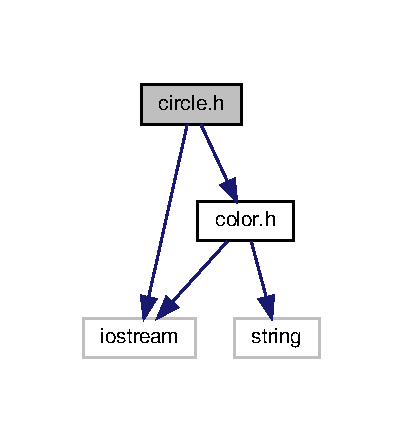
\includegraphics[width=194pt]{circle_8h__incl}
\end{center}
\end{figure}
\subsection*{Classes}
\begin{DoxyCompactItemize}
\item 
class \hyperlink{classCircle}{Circle}
\end{DoxyCompactItemize}
\subsection*{Functions}
\begin{DoxyCompactItemize}
\item 
std\+::ostream \& \hyperlink{circle_8h_ae8c7ccd438b4cffe3c29aebfdd0a73b0}{operator$<$$<$} (std\+::ostream \&stream, const \hyperlink{classCircle}{Circle} \&circle)
\begin{DoxyCompactList}\small\item\em Overload of the output stream to display a circle. \end{DoxyCompactList}\end{DoxyCompactItemize}


\subsection{Function Documentation}
\mbox{\Hypertarget{circle_8h_ae8c7ccd438b4cffe3c29aebfdd0a73b0}\label{circle_8h_ae8c7ccd438b4cffe3c29aebfdd0a73b0}} 
\index{circle.\+h@{circle.\+h}!operator$<$$<$@{operator$<$$<$}}
\index{operator$<$$<$@{operator$<$$<$}!circle.\+h@{circle.\+h}}
\subsubsection{\texorpdfstring{operator$<$$<$()}{operator<<()}}
{\footnotesize\ttfamily std\+::ostream\& operator$<$$<$ (\begin{DoxyParamCaption}\item[{std\+::ostream \&}]{stream,  }\item[{const \hyperlink{classCircle}{Circle} \&}]{circle }\end{DoxyParamCaption})}



Overload of the output stream to display a circle. 


\begin{DoxyParams}{Parameters}
{\em stream} & \\
\hline
{\em circle} & \\
\hline
\end{DoxyParams}
\begin{DoxyReturn}{Returns}
The stream 
\end{DoxyReturn}

\hypertarget{color_8h}{}\section{color.\+h File Reference}
\label{color_8h}\index{color.\+h@{color.\+h}}
{\ttfamily \#include $<$iostream$>$}\newline
{\ttfamily \#include $<$string$>$}\newline
Include dependency graph for color.\+h\+:\nopagebreak
\begin{figure}[H]
\begin{center}
\leavevmode
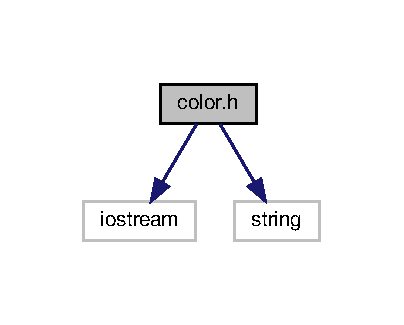
\includegraphics[width=194pt]{color_8h__incl}
\end{center}
\end{figure}
This graph shows which files directly or indirectly include this file\+:\nopagebreak
\begin{figure}[H]
\begin{center}
\leavevmode
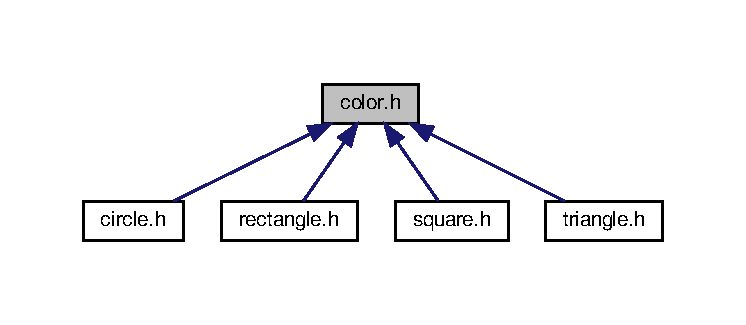
\includegraphics[width=350pt]{color_8h__dep__incl}
\end{center}
\end{figure}
\subsection*{Classes}
\begin{DoxyCompactItemize}
\item 
class \hyperlink{classColor}{Color}
\end{DoxyCompactItemize}
\subsection*{Functions}
\begin{DoxyCompactItemize}
\item 
std\+::string \hyperlink{color_8h_a9ad55674d017a8df8a29f60fe160b762}{to\+String} (const \hyperlink{classColor_a20a7b04657c1d83fae5d54514d3f1622}{Color\+::\+Code} \&code)
\begin{DoxyCompactList}\small\item\em Convert the code color in a string. \end{DoxyCompactList}\item 
std\+::ostream \& \hyperlink{color_8h_a2949bc642f18dffe591014eca1260be5}{operator$<$$<$} (std\+::ostream \&stream, const \hyperlink{classColor}{Color} \&color)
\begin{DoxyCompactList}\small\item\em Overload of the output sream to display a color. \end{DoxyCompactList}\end{DoxyCompactItemize}


\subsection{Function Documentation}
\mbox{\Hypertarget{color_8h_a2949bc642f18dffe591014eca1260be5}\label{color_8h_a2949bc642f18dffe591014eca1260be5}} 
\index{color.\+h@{color.\+h}!operator$<$$<$@{operator$<$$<$}}
\index{operator$<$$<$@{operator$<$$<$}!color.\+h@{color.\+h}}
\subsubsection{\texorpdfstring{operator$<$$<$()}{operator<<()}}
{\footnotesize\ttfamily std\+::ostream\& operator$<$$<$ (\begin{DoxyParamCaption}\item[{std\+::ostream \&}]{stream,  }\item[{const \hyperlink{classColor}{Color} \&}]{color }\end{DoxyParamCaption})}



Overload of the output sream to display a color. 


\begin{DoxyParams}{Parameters}
{\em stream} & \\
\hline
{\em color} & \\
\hline
\end{DoxyParams}
\begin{DoxyReturn}{Returns}
The stream 
\end{DoxyReturn}
\mbox{\Hypertarget{color_8h_a9ad55674d017a8df8a29f60fe160b762}\label{color_8h_a9ad55674d017a8df8a29f60fe160b762}} 
\index{color.\+h@{color.\+h}!to\+String@{to\+String}}
\index{to\+String@{to\+String}!color.\+h@{color.\+h}}
\subsubsection{\texorpdfstring{to\+String()}{toString()}}
{\footnotesize\ttfamily std\+::string to\+String (\begin{DoxyParamCaption}\item[{const \hyperlink{classColor_a20a7b04657c1d83fae5d54514d3f1622}{Color\+::\+Code} \&}]{code }\end{DoxyParamCaption})}



Convert the code color in a string. 


\begin{DoxyParams}{Parameters}
{\em code} & \\
\hline
\end{DoxyParams}
\begin{DoxyReturn}{Returns}
The color in string 
\end{DoxyReturn}

\hypertarget{rectangle_8h}{}\section{rectangle.\+h File Reference}
\label{rectangle_8h}\index{rectangle.\+h@{rectangle.\+h}}
{\ttfamily \#include $<$iostream$>$}\newline
{\ttfamily \#include \char`\"{}color.\+h\char`\"{}}\newline
Include dependency graph for rectangle.\+h\+:\nopagebreak
\begin{figure}[H]
\begin{center}
\leavevmode
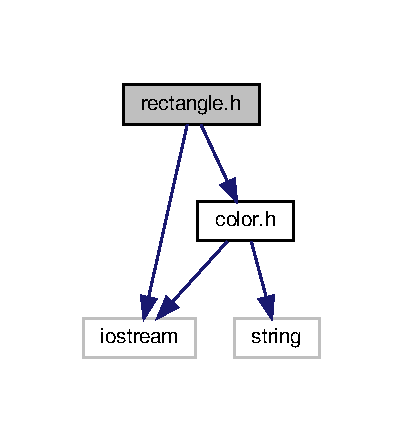
\includegraphics[width=194pt]{rectangle_8h__incl}
\end{center}
\end{figure}
\subsection*{Classes}
\begin{DoxyCompactItemize}
\item 
class \hyperlink{classRectangle}{Rectangle}
\end{DoxyCompactItemize}
\subsection*{Functions}
\begin{DoxyCompactItemize}
\item 
std\+::ostream \& \hyperlink{rectangle_8h_a369ab6fb09fcf531a4738b328840d0ec}{operator$<$$<$} (std\+::ostream \&stream, const \hyperlink{classRectangle}{Rectangle} \&rectangle)
\begin{DoxyCompactList}\small\item\em Overload of the output stream to display a rectangle. \end{DoxyCompactList}\end{DoxyCompactItemize}


\subsection{Function Documentation}
\mbox{\Hypertarget{rectangle_8h_a369ab6fb09fcf531a4738b328840d0ec}\label{rectangle_8h_a369ab6fb09fcf531a4738b328840d0ec}} 
\index{rectangle.\+h@{rectangle.\+h}!operator$<$$<$@{operator$<$$<$}}
\index{operator$<$$<$@{operator$<$$<$}!rectangle.\+h@{rectangle.\+h}}
\subsubsection{\texorpdfstring{operator$<$$<$()}{operator<<()}}
{\footnotesize\ttfamily std\+::ostream\& operator$<$$<$ (\begin{DoxyParamCaption}\item[{std\+::ostream \&}]{stream,  }\item[{const \hyperlink{classRectangle}{Rectangle} \&}]{rectangle }\end{DoxyParamCaption})}



Overload of the output stream to display a rectangle. 


\begin{DoxyParams}{Parameters}
{\em stream} & \\
\hline
{\em rectangle} & \\
\hline
\end{DoxyParams}
\begin{DoxyReturn}{Returns}
The stream 
\end{DoxyReturn}

\hypertarget{square_8h}{}\section{square.\+h File Reference}
\label{square_8h}\index{square.\+h@{square.\+h}}
{\ttfamily \#include $<$iostream$>$}\newline
{\ttfamily \#include \char`\"{}color.\+h\char`\"{}}\newline
Include dependency graph for square.\+h\+:\nopagebreak
\begin{figure}[H]
\begin{center}
\leavevmode
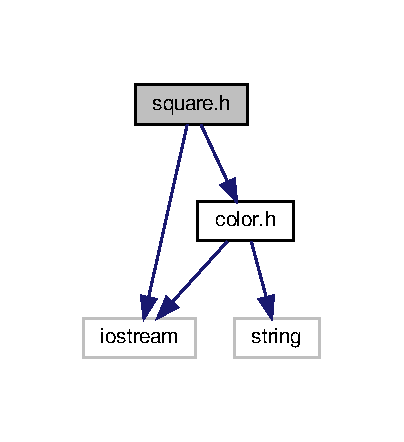
\includegraphics[width=194pt]{square_8h__incl}
\end{center}
\end{figure}
\subsection*{Classes}
\begin{DoxyCompactItemize}
\item 
class \hyperlink{classSquare}{Square}
\end{DoxyCompactItemize}
\subsection*{Functions}
\begin{DoxyCompactItemize}
\item 
std\+::ostream \& \hyperlink{square_8h_a3e24e247af4633a422b1e11dd1aa4570}{operator$<$$<$} (std\+::ostream \&stream, const \hyperlink{classSquare}{Square} \&square)
\begin{DoxyCompactList}\small\item\em Overload of the output stream to display a square. \end{DoxyCompactList}\end{DoxyCompactItemize}


\subsection{Function Documentation}
\mbox{\Hypertarget{square_8h_a3e24e247af4633a422b1e11dd1aa4570}\label{square_8h_a3e24e247af4633a422b1e11dd1aa4570}} 
\index{square.\+h@{square.\+h}!operator$<$$<$@{operator$<$$<$}}
\index{operator$<$$<$@{operator$<$$<$}!square.\+h@{square.\+h}}
\subsubsection{\texorpdfstring{operator$<$$<$()}{operator<<()}}
{\footnotesize\ttfamily std\+::ostream\& operator$<$$<$ (\begin{DoxyParamCaption}\item[{std\+::ostream \&}]{stream,  }\item[{const \hyperlink{classSquare}{Square} \&}]{square }\end{DoxyParamCaption})}



Overload of the output stream to display a square. 


\begin{DoxyParams}{Parameters}
{\em stream} & \\
\hline
{\em square} & \\
\hline
\end{DoxyParams}
\begin{DoxyReturn}{Returns}
The stream 
\end{DoxyReturn}

\hypertarget{triangle_8h}{}\section{triangle.\+h File Reference}
\label{triangle_8h}\index{triangle.\+h@{triangle.\+h}}
{\ttfamily \#include $<$iostream$>$}\newline
{\ttfamily \#include \char`\"{}color.\+h\char`\"{}}\newline
Include dependency graph for triangle.\+h\+:\nopagebreak
\begin{figure}[H]
\begin{center}
\leavevmode
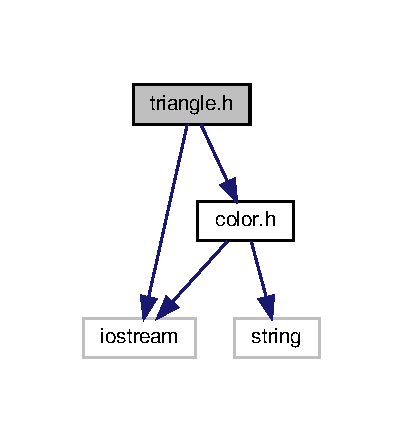
\includegraphics[width=194pt]{triangle_8h__incl}
\end{center}
\end{figure}
\subsection*{Classes}
\begin{DoxyCompactItemize}
\item 
class \hyperlink{classTriangle}{Triangle}
\end{DoxyCompactItemize}
\subsection*{Functions}
\begin{DoxyCompactItemize}
\item 
std\+::ostream \& \hyperlink{triangle_8h_a5de1287ddcd8434e652168aff42b7636}{operator$<$$<$} (std\+::ostream \&stream, const \hyperlink{classTriangle}{Triangle} \&triangle)
\end{DoxyCompactItemize}


\subsection{Function Documentation}
\mbox{\Hypertarget{triangle_8h_a5de1287ddcd8434e652168aff42b7636}\label{triangle_8h_a5de1287ddcd8434e652168aff42b7636}} 
\index{triangle.\+h@{triangle.\+h}!operator$<$$<$@{operator$<$$<$}}
\index{operator$<$$<$@{operator$<$$<$}!triangle.\+h@{triangle.\+h}}
\subsubsection{\texorpdfstring{operator$<$$<$()}{operator<<()}}
{\footnotesize\ttfamily std\+::ostream\& operator$<$$<$ (\begin{DoxyParamCaption}\item[{std\+::ostream \&}]{stream,  }\item[{const \hyperlink{classTriangle}{Triangle} \&}]{triangle }\end{DoxyParamCaption})}

Overload of the output stream to display a triangle 
\begin{DoxyParams}{Parameters}
{\em stream} & \\
\hline
{\em triangle} & \\
\hline
\end{DoxyParams}
\begin{DoxyReturn}{Returns}
The stream 
\end{DoxyReturn}

%--- End generated contents ---

% Index
\backmatter
\newpage
\phantomsection
\clearemptydoublepage
\addcontentsline{toc}{chapter}{Index}
\printindex

\end{document}
